\documentclass[12pt]{article}
\usepackage[english]{babel}
\usepackage[utf8x]{inputenc}
\usepackage{amsmath}
\usepackage{amssymb}
\usepackage{graphicx}
\usepackage{textcomp}
\usepackage{hyperref}
\usepackage[colorinlistoftodos]{todonotes}
\usepackage{xcolor}

\hypersetup{
    colorlinks,
    linkcolor={blue!50!black},
    citecolor={blue!50!black},
    urlcolor={blue!80!black}
}

\newcommand{\textapprox}{\raisebox{0.5ex}{\texttildelow}}
\newcommand\tab[1][1cm]{\hspace*{#1}}
\newcommand{\ET}{\mathcal{E}}
\newcommand{\R}{\mathbb{R}}
\begin{document}

\begin{titlepage}

\newcommand{\HRule}{\rule{\linewidth}{0.5mm}} % Defines a new command for the horizontal lines, change thickness here


\center % Center everything on the page
 
%----------------------------------------------------------------------------------------
%	HEADING SECTIONS
%----------------------------------------------------------------------------------------

\textsc{\LARGE Indian Institute of Technology Bombay}\\[1cm] % Name of your university/college
\textsc{\Large Department of Computer Science \& Engineering}\\[0.5cm] % Major heading such as course name
\textsc{\large RnD Report}\\[0.5cm] % Minor heading such as course title

%----------------------------------------------------------------------------------------
%	TITLE SECTION
%----------------------------------------------------------------------------------------

\HRule \\[0.4cm]
{ \huge \bfseries Word, Entity and Knowledge Graph Embeddings}\\[0.4cm] % Title of your document
\HRule \\[1.5cm]
 
%----------------------------------------------------------------------------------------
%	AUTHOR SECTION
%----------------------------------------------------------------------------------------

\begin{minipage}{0.4\textwidth}
\begin{flushleft} \large
\emph{Author:}\\
Rishabh Agarwal % Your name
\end{flushleft}
\end{minipage}
~
\begin{minipage}{0.4\textwidth}
\begin{flushright} \large
\emph{Supervisor:} \\
Prof. Soumen Chakrabarti % Supervisor's Name
\end{flushright}
\end{minipage}\\[2cm]

% If you don't want a supervisor, uncomment the two lines below and remove the section above
%\Large \emph{Author:}\\
%John \textsc{Smith}\\[3cm] % Your name

%----------------------------------------------------------------------------------------
%	DATE SECTION
%----------------------------------------------------------------------------------------

{\large \today}\\[2cm] % Date, change the \today to a set date if you want to be precise

%----------------------------------------------------------------------------------------
%	LOGO SECTION
%----------------------------------------------------------------------------------------


\includegraphics[height=3.8cm,keepaspectratio]{logo.jpg}\\[0cm] % Include a department/university logo - this will require the graphicx package
 
%----------------------------------------------------------------------------------------

\vfill % Fill the rest of the page with whitespace

\end{titlepage}


\tableofcontents
\pagebreak

% \begin{abstract}
% Learning quickly is a hallmark of human intelligence, whether it involves recognizing objects from a few examples or quickly learning new skills after just minutes of experience. One of the current limitations of deep learning is the need for tremendous amounts of data.
% Finding techniques to achieve state-of-the-art performance on tasks with orders of magnitude less data is a very active research area. In this work, we survey some of the recent approaches to tackle this problem of learning new concepts rapidly with very little data.
% \end{abstract}

\section{Introduction}

Recently, word embeddings have been exceptionally successful in many NLP tasks. In fact, in many NLP architectures, they have almost completely replaced traditional distributional features such as Brown clusters and LSA features.\\

Semantic relations between word embeddings seem nothing short of magical to the uninitiated and Deep Learning NLP talks frequently prelude with the notorious \textit{king − man + woman ≈ queen} slide, word embeddings are possibly the primary reason for NLP's breakout recently.\\

There has already been a lot of work in the quest for the best embedding models. Lately,  there has been lot of papers explaining why such embedding models work and need for better formulation of such models. This work summarizes my study on word embeddings, embeddings for knowledge graphs and entity embeddings.

\section{Word embedding models}

It is estimated that number of tokens in the English language is in millions. Are these tokens unrelated? No. Thus, we want to encode word tokens each into some vector that represents a point in some sort of ``word" space. According to me, the most intuitive reason is that perhaps there actually exists some N-dimensional space (such that N $<<$ 1 million) that is sufficient to encode all semantics of our language. Each dimension would encode some meaning that we transfer using speech.\newline

The simplest and the most naive method is to represent each word as an independent one-hot vector. This word representation does not give us directly any notion of similarity and uses up a lot of space (each embedding is a vector which belongs to $\R^{|V|}$ where V is the size of the vocabulary).\\

To mitigate these problems, various embedding models were developed. In all such methods, the word vector is a succinct representation of the distribution of other words around this word. This is also asserted by the famous Firth’s hypothesis from 1957, ``You shall know a word by the company it keeps.". 
The word2vec\cite{DBLP:journals/corr/abs-1301-3781} and GloVe\cite{Pennington14glove:global} are the currently used embedding models. You can read more about them on this blog\cite{ruder_2016}.\newline

The word2vec papers are a bit mysterious, and have motivated much followup work. A paper\cite{NIPS2014_5477} by Levy and Goldberg explains that the word2vec methods are actually modern versions of older vector space methods. \newline

Arora et al.\cite{DBLP:journals/corr/AroraLLMR15} also tried to provide a theoretical justification for nonlinear models like PMI, word2vec, and GloVe. It also helps explain why low-dimensional semantic embeddings contain linear algebraic structure that allows solution of word analogies.\newline

In the next sections, we'll discuss about the various extensions for the embeddings.

\section{Contextual Embeddings}
Since we want to use word embeddings for downstream NLP tasks, we can't ignore polysemy and thus a word should have multiple embeddings depending on it's meaning. A lot of work has already been done for learning word embeddings for multiple senses corresponding to a word!\\

A large number of research papers such as sense2vec\cite{DBLP:journals/corr/TraskML15} assumes the training corpora is present with Part-of-speech(POS)/Word-sense disambiguation (WSD) annotations. Another large cluster assumes no such supervision of POS/WSD. Some of those papers regard sense as a discrete latent label that is inferred to perform the training.\\

Arvind et al.\cite{DBLP:journals/corr/NeelakantanSPM15} learned multiple embeddings per word jointly performing word sense discrimination and embedding learning, by non-parametrically estimating the number of senses per word type.\\

So, the vector embedding of a word should not be a single vector but should depend on the context in which the word is present. Therefore, ideally we need a formulation in which we are presented a generic function function 
f(. , .) which takes two argument, one corresponding to the word and other for its context and returns the context-dependent word-embedding. Elegant formulation of contextual embeddings is a novel area to pursue.\\

\section{L2-Embeddings}
A natural question which arises is : What if we use L2-Distance as a similarity measure rather than cosine similarity? In L2-embeddings, instead of maximizing the cosine similarity between a word and its context vectors, we minimize the L2 distance between them. One simple motivation for doing that is we want similar words to lie close to each other in the embedding space.\\ 

Suppose, if we are able to obtain such embeddings, then how do we test the goodness of such embeddings? The usual analogy tests as performed in word2vec won't work.\\

Suppose we are given words x, y and z. When word2vec wants to find the word w which is to x as y is to z, it is trying to find w maximizing the dot product \textit{D = w. (x + y – z)} .But this is the same thing as maximizing \textit{w.x + w.y – w.z} .In other words, what D is really doing is saying ``Show me words which are similar to x and y but are dissimilar to z.''\\ 

Levy et al.\cite{Levy14linguisticregularities} showed that this is indeed the case by proving that their 3COSMUL objective works better for analogy tests.
From this point of view, it is hypothesized that minimizing $( ||w-x|| * ||w-y|| ) / ||w-z||$ with respect to w would find the words w such that w:x :: y:z

\section{Embeddings for Knowledge Graph}
Web-scale knowledge graph(KGs) provide a structured representation of world knowledge. They enable wide range of applications including recommender systems, question answering and automated. The incompleteness of these knowledge graphs, has stimulated research into predicting missing entries, a task known as knowledge graph completion. \\

Recently, vector space embeddings of KGs have received considerable attention, as they can be used to create statistical models of entire KGs
and therefore knowledge graph completion

\subsection{Compositional Vector Space Models}
Let E denote the set of all entities and P the set of all relation types(predicates) in a domain. A binary relation is a subset $R_p \subseteq \ET  \, X \, \ET$ of all pairs of entities (i.e. those pairs which are in a relation of type p). Higher-arity relations are defined analogously. The characteristic function $\phi_p :\ET X \ET \rightarrow \{ \pm 1\}$ of a relation $R_p$ indicates for each possible pair of entities whether they are part of $R_p$. We will denote (possible) relation instances as $R_p(s, o)$, where s, o $\epsilon \space \ET$ denote the first and second argument of the asymmetric relation $R_p$. We will refer to s, o as subject and object and to $R_p(s, o)$ as triples.

Here we discuss models of the form:
$$ Pr(\phi_p(s,o) =1|\Theta) = \sigma(\eta_{spo})  = \sigma(\textbf{r}^T_p(\textbf{e}_s\, o \, \textbf{e}_o)) \qquad (1) $$

where $r_p\, \epsilon \, \R^{d_r} , e_i \, \epsilon \, \R_{d_e}$ are vector representations of relations and entities; $\sigma$ denotes the sigmoid function; $ \Theta = \{e_i\}^{n_e}_1 \,\cup\, \{r_k\}^{n_k}_1$ denotes the set of all embeddings;
$ o : \R^{d_e} \, X \, R^{d_e} \rightarrow \R^{d_p}$ denotes the compositional operator which creates a composite vector representation for the pair(s,o)from the embeddings $\textbf{e}_s, \textbf{e}_o$. 

Let $x_i \,\epsilon\,  \mathcal{P} X \ET X \ET$ denote a triple , and $y_i \, \epsilon\, \{ \pm 1 \}$ denote its label. Given a dataset $D =\{f(x_i, y_i)\}^m_{i=1}$ of true and false relation instances, we then want to learn representations of entities and relations that best explain D according to eq. (1).

\begin{figure}
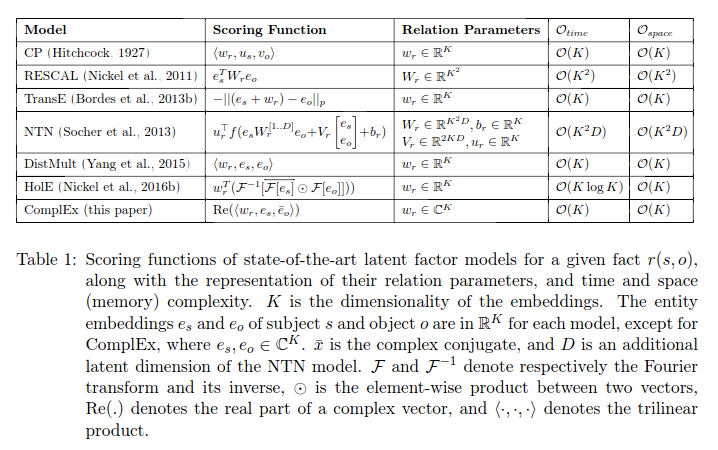
\includegraphics[width=\textwidth,keepaspectratio]{models.png}
\end{figure}

Existing models for knowledge graphs are based on the following compositional operators:

\subsubsection*{Tensor Product} 
Given entity embeddings $\textbf{a}, \textbf{b} \, \epsilon\, \R^d$ , tensor product models represent pairs of entities via $\textbf{a} \,o\,\textbf{b} = \textbf{a} \otimes  \textbf{b} \,\epsilon\,R^{d^2}$ \newline
RESCAL\cite{Nickel_athree-way} is one such compositional models which uses the tensor product. While the tensor product allows to capture rich interactions, its main problem as a compositional operator lies in the fact that it requires a large number of parameters.

\subsubsection{Holographic Embeddings(HoLE)}
Nickel et al.\cite{DBLP:journals/corr/NickelRP15} developed this model. Here the compositional operator used is the  circular correlation of vectors to represent pairs of entities, i.e 
$$ \textbf{a} \,o\, \textbf{b} = \textbf{a} \star \textbf{b} $$
where $ \star : \R^d \,X\, \R^d \rightarrow \R^d $ denotes circular correlation\cite{} :
$$ [\textbf{a} \star \textbf{b}]_k = \sum_{i=0}^{d-1} a_i\, b_{(k+i)mod\,d} $$

As a compositional operator, circular correlation can be
interpreted as a compression of the tensor product.

\phantomsection
\label{neural}
A natural thought that arises is that we can simply use a generic neural network using the embeddings $\textbf{e}_s, \textbf{e}_r$ as input to the network which generate O(d) (let's say 2d) features  instead of the circular correlation which is supposed to work even better.

\subsubsection{ComplEx Embeddings}
The idea of this paper\cite{DBLP:journals/corr/TrouillonWRGB16} was to use two embeddings for a entity instead of one, and they represented those two two embeddings with a complex valued vector. 
\begin{align*}
\eta_{sro} = \phi_r(s, o; \Theta) &= Re(\textbf{e}_s \textbf{W}_r \textbf{e}_o)\\
 &= Re(\sum^{K}_{k=1}w_{rk}e_{sk}\bar{e}_{ok})\\
 &= Re(\langle w_r , e_s, \bar{e}_o  \rangle )
\end{align*}
where $\sigma(\eta_{sro})$ denotes the probability that r(s, o) is true.
Here $Re<\cdot>$ denotes the real part of a imaginary vector. Also,  $e_s, e_o\, \epsilon \, \mathbb{C}_K$
are the rows in E corresponding to the entities s and o; $w_r = diag(W_r) \, \epsilon \, \mathbb{C}_K$ is a complex vector.
\begin{align*}
Re(\langle w_r , e_s, \bar{e}_o  \rangle ) &= \langle Re(w_r), Re(e_s), Re(e_o) \rangle \\
&+ \langle Re(w_r), Im(e_s), Im(e_o) \rangle \\
&+ \langle Im(w_r), Re(e_s), Im(e_o) \rangle \\
&- \langle Im(w_r), Im(e_s), Im(e_o) \rangle \\
\end{align*}

These embeddings can model both symmetric and antisymmetric relations. Although, this model just identifies  another possible way to find interactions between two embeddings. The neural network approach as mentioned \hyperref[neural]{here} is even more generic.

\section{Entity Embeddings}
\label{entity}
Conceptual spaces are geometric representations of conceptual knowledge, in which entities correspond
to points, natural properties correspond to
convex regions, and the dimensions of the space
correspond to salient features. While conceptual
spaces enable elegant models of various cognitive
phenomena, the lack of automated methods for
constructing such representations have so far limited
their application in artificial intelligence.\newline

Jameel et al.\cite{DBLP:conf/coling/JameelS16} proposed a method in which they learnt a vector-space embedding of entities from Wikipedia and constrained this embedding such that entities of the same semantic type are located in
some lower-dimensional subspace using nuclear norm\cite{2007arXiv0706.4138R} regularization.
The model they proposed has the following form:
$$ J = \alpha J_{text} + (1 − \alpha)(J_{type} + J_{rel}) + \beta J_{reg}$$

Component $J_{text}$ will be used to constrain the representation
of the entities based on their textual description,
$J_{type}$ will impose the constraint that entities of the same type
belong to a particular subspace, $J_{rel}$ will use the relations in R to improve the alignment between these subspaces, and $J_{reg}$ is a regularization component which will allow the model to automatically select the most appropriate number of dimensions for every subspace.\\

This model is penalizing loss function $J_{type}$ by a global variable $\alpha$ instead of using different $\alpha$ values for different types.
The authors of this paper\cite{} point out that nuclear
norm regularization allows their model to automatically
select the most appropriate number of dimensions for the subspace
corresponding to each type. So, can we constraint embeddings in bounded regions using this method?  This is one such question which should be investigated experimentally.\\

Bouraoui et al.\cite{DBLP:conf/aaai/BouraouiJS17} proposed a new method for inductive reasoning with ontologies which consisted of using a form of
Bayesian inference over interpretable feature representations
that are obtained from a learned vector space embedding using the method as proposed \hyperref[entity]{above}. Though the idea of this paper was nice, there were a lot of assumptions that seem to be over-simplifying the problem of knowledge base completion.\\

Recently, Yamada et al\cite{DBLP:journals/corr/YamadaS0T16},  proposed a novel embedding method specifically designed for Named Entity Disambiguation. The proposed method jointly maps words and entities into the same continuous vector space. The method extends the skip-gram model by using two models. The KB graph model learns the relatedness of entities using the link structure of the KB, whereas the anchor context model aims to align vectors such that similar words and entities occur close to one another in the vector space by leveraging KB anchors and their context words.

\section{Conclusion}
We discussed a lot of possible extensions for the existing embedding models and raised some questions which are still unanswered. The next logical step is to try out those ideas and find answers to some of the questions we raised!

\bibliographystyle{unsrt}
\addtocounter{section}{1}
\addcontentsline{toc}{section}{Bibliography}
\bibliography{report}

\end{document}